%!TEX root = ../report.tex
\clearpage
\section{Hardware Description}
\label{sec:hardware-description}
% Mention the difference between previous chapter
This section gives an outline of the hardware implemented in this system. This section also elaborates on hardware decisions.

\subsection{Storage cluster}
\label{subsec:database-data}
HEMS will use clusters of computer to manage the database system and to store our data. The cluster enables the database to replicate data. This means no backup is needed, the data is always available in multiple servers. Furthermore, user account information is hashed using bcrypt after being salted with 128 randomly generated characters to increase security. The cluster will also be accessible by the main analytics part as the data will come and go through the main analytics part. The logical schematic of the storage cluster is depicted in \autoref{fig:database-cluster}

\begin{figure}[H]
\centering
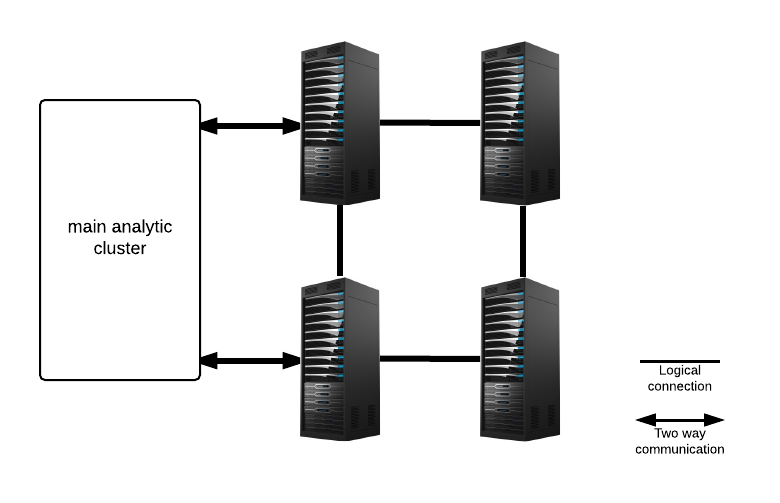
\includegraphics[width=0.7\textwidth]{6-hardware/images/db-cluster.png}
\caption{Logical schematic of storage cluster of HEMS}
\label{fig:database-cluster}
\end{figure}

As can be seen in \autoref{fig:database-cluster}, HEMS will use four database racks to have redundancy in the system. The server is connected as a ring, which is the common way to setup database server. By using this form of architecture, HEMS will be more reliable and fault tolerant. There will also be two physical connection to the main analytic cluster to make this system more fault tolerant in terms of connection. HEMS database cluster will use the same server, Dell PowerEdge R530, for controlling the SATA storage machine.

\subsection*{Related patterns}
This storage cluster implements broker, shared repository, and unit of work patterns. Broker pattern is implemented in a mechanism that any other component of this system can connect to the cluster and see this as a single entity, although actually the cluster consists of more than one entity. If this storage cluster is seen as a single entity, then this is also an implementation of shared repository pattern, where a client or other instance connects to the storage cluster and proceeds with corresponding operations. Unit of Work pattern will be used to keep track of changes to objects and to coordinate writing these changes to the database in one database call.

\subsection{Compute cluster}
\label{subsec:analytics}
Compute cluster will be the main brain of HEMS. The data presentation will be handled by this system. The analysis process also runs on top of this hardware. To increase availability and reliability, HEMS will have six server racks to do the processing as depicted in \autoref{fig:analytic-cluster}.

\begin{figure}[H]
\centering
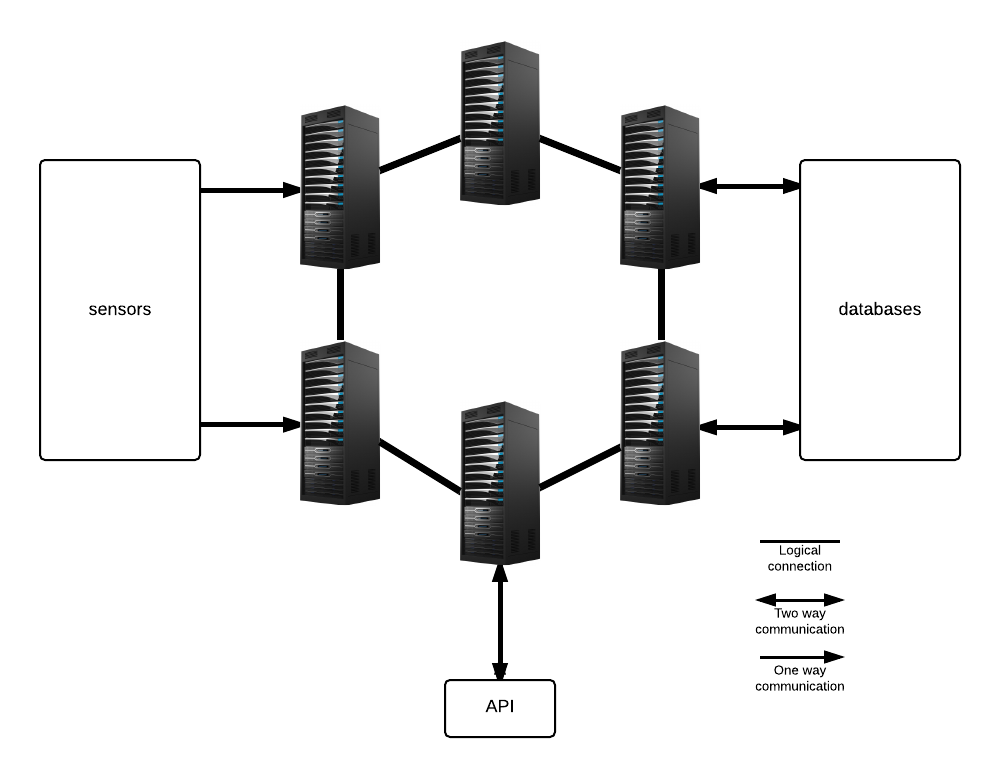
\includegraphics[width=0.7\textwidth]{6-hardware/images/analytic-cluster.png}
\caption{Logical schematic of analytic cluster of HEMS}
\label{fig:analytic-cluster}
\end{figure}

\subsection*{Related patterns}
Front page controller pattern is implemented in the compute cluster, which includes decorator and command pattern, because the compute cluster is also responsible for handling incoming connection through API. 